\documentclass[12pt, bibliography=totocnumbered]{scrartcl}
\usepackage{config}
\usepackage[ngerman]{babel}
\renewcaptionname{ngerman}{\figurename}{Abb.}
\renewcaptionname{ngerman}{\tablename}{Tab.}
\sisetup{locale = DE}

%\usepackage[english]{babel}


\newcommand{\VERSUCHSNAME}{Polykondensation und Polyaddition}
\newcommand{\Versuchsdatum}{14.03.2025}
\newcommand{\Assistent}{Dr. Dongren Wang}


\newcommand{\VerfasserEINS}{Sven Wacker}
\newcommand{\MailEINS}{st182535@stud.uni-stuttgart.de}
\newcommand{\MatrikelnummerEINS}{3645844}
\newcommand{\VerfasserZWEI}{Leon Ayasse}
\newcommand{\MailZWEI}{st182275@stud.uni-stuttgart.de}
\newcommand{\MatrikelnummerZWEI}{3645857}
\newcommand{\PROTOKOLLDATUM}{\today}
\newcommand{\VerfasserDREI}{Jan Wolf}
\newcommand{\MailDREI}{st183650@stud.uni-stuttgart.de}
\newcommand{\MatrikelnummerDREI}{3652905}

\begin{document}
\begin{titlepage}
    \begin{center}
        \Huge{\textbf{\VERSUCHSNAME}}\\
        \vspace{10mm}
        \huge{Protokoll zur Laborpraktischen Übung Polymerchemie}\\
        \vspace{10mm}
        \Large{Universität Stuttgart}\\
    \end{center}
    \begin{center}
        Stuttgart, den \PROTOKOLLDATUM
    \end{center}
    \vspace{10mm}
    \begin{center}
        \begin{tabular}{ll}
            \large{Verfasser:}     & \large{\VerfasserEINS}~\large{(\MatrikelnummerEINS)} \\
                                   & \large{\MailEINS}                                    \\
                                   &                                                      \\
                                   & \large{\VerfasserZWEI}~\large{(\MatrikelnummerZWEI)} \\
                                   & \large{\MailZWEI}                                    \\
                                   &                                                      \\
                                   & \large{\VerfasserDREI}~\large{(\MatrikelnummerDREI)} \\
                                   & \large{\MailDREI}                                    \\
                                   &                                                      \\
            \large{Assistent:}     & \large{\Assistent}                                   \\
                                   &                                                      \\
            \large{Versuchsdatum:} & \large{\Versuchsdatum}                               \\
        \end{tabular}
    \end{center}
\end{titlepage}
\tableofcontents
\thispagestyle{empty}
\newpage
\setcounter{page}{1}
\section{Theoretische Grundlagen}
\subsection{Polykondensationen}
Bei einer Kondensationsreaktion reagieren zwei funktionelle Gruppen zweier Moleküle oder desselben Moleküls unter Abspaltung von kleineren Molekülen wie Wasser, Ammoniak oder HCl miteinander. Bei einer Polykondensationsreaktion wird diese Reaktion vermehrt mit solchen Molekülen unter mehrfacher Abspaltung durchgeführt. Beliebte Monomere sind Dicarbonsäuren, Diamine oder auch Dialkohole. Es werden zwei Arten von Reaktionen unterschieden. Einerseits gibt es AA/BB-Reaktionen, bei denen zwei verschiedene Monomere mit jeweils gleichen Endgruppen miteinander reagieren, beispielsweise Dicarbonsäuren mit Dialkoholen zum jeweiligen Ester oder Diester. Und andererseits die AB-Reaktionen, bei welchen eine Monomerart mit zwei verschiedenen Endgruppen mit sich selbst oder anderen Monomeren reagieren kann. Beide Reaktionsarten fallen unter die Kategorie der Stufenwachstumsreaktionen, welche zunächst Oligomere mit den funktionellen Gruppen der verwendeten Monomere oder des verwendeten Monomers an ihren Enden aufweisen. Diese können nun mit anderen Oligomeren, anderen Monomeren oder mit sich selbst unter Ringschluss reagieren. Die drei möglichen Reaktionen stehen dabei im Gleichgewicht miteinander. Außerdem können neben dem Wachstum der Hauptkette auch Seitenkettenreaktionen an funktionellen Stellen des backbones  wie Umesterungen oder Transamidierungen auftreten. Dies führt zu teils hochvernetzten Polymeren. 
\subsection{Polyadditionen}
Polyadditionen unterscheiden sich im Wesentlichen von den Polykondensationen, indem sie keine kleineren Moleküle bei der Polymerisation abspalten. Auch sie zählen zu den Stufenwachstumsreaktionen. Über Polyaddition werden meist Polyurethane aus Diolen und Diisocyanaten hergestellt. Um quervernetzte Polymere zu erhalten, können auch Hydroxyverbindungen und Isocyanate mit mehr als zwei funktionellen Gruppen eingesetzt werden. Dabei bleibt die Reaktivität der Di-, Oligo- oder Polymere meist gleich der der Monomere. Polyurethane können während der Polymerisierung bei Anwesenheit von Wasser unter Abspaltung von $\mathrm{CO_2}$ zu sogenannten PU-Schäumen geschäumt werden. Es wird zwischen Weichschäumen mit beweglichen Kettengliedern und Hartschäumen mit kurzen hochverzweigten Kettengliedern unterschieden. Weichschäume werden oft mit $\mathrm{CO_2}$ oder niedermolekularen Alkanen wie Propan oder Pentan geschäumt, während Hartschäume mit niedrigsiedenden inerten Treibmitteln geschäumt werden. Um die Reaktionsgeschwindigkeit zu beschleunigen, werden oft sterisch gehinderte organische Basen wie 1,4-Diazabicyclo[2.2.2]oktan oder organometallische Verbindungen wie Dibutylzinndilaurat eingesetzt. Diese ermöglichen einen alternativen Reaktionsmechanismus, welcher in Abbildung \ref{fig:Polyaddition_Katalysator} dargestellt ist:
\begin{figure}[H]
    \centering
    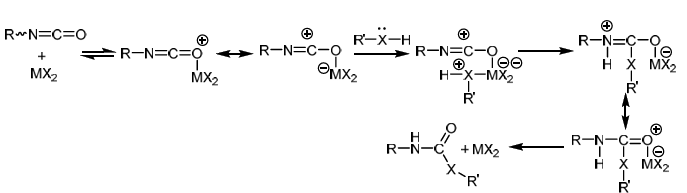
\includegraphics[width=0.8\linewidth]{Abbildungen/Polyaddition_Katalysator.png}
    \caption{Reaktionsmechanismus der Polyaddition unter Verwendung eines Katalysators.}
    \label{fig:Polyaddition_Katalysator}
\end{figure}

\subsection{Kinetik von Stufenwachstumsreaktionen}
Sowohl bei der Polyaddition als auch bei der Polykondensation spielt das molare Verhältnis der verwendeten Monomere eine essentielle Rolle im Bezug auf den Polymerisationsgrad. Im Folgenden wird die Kinetik dieser Reaktionen anhand der Polykondensation dargestellt. Bei diesem Reaktionstyp ist die säurekatalysierte Veresterung des Alkohols mit der Carbonsäure der geschwindigkeitsbestimmende Schritt. Dieser kann mithilfe eines Katalysators K beschleunigt werden. Dabei ist die Reaktionsgeschwindigkeit proportional zu den Konzentrationen aller drei Komponenten. Da äquimolare Verhältnisse von Alkohol und Carbonsäure unabdingbar für diese Reaktion sind, gilt:
\begin{equation}
[\mathrm{COOH}]=[\mathrm{OH}]=c    
\end{equation}
Aus den davor besprochenen Verhältnissen ergibt sich:
\begin{equation}
-\frac{\mathrm{d}c}{\mathrm{d}t}=k\cdot\mathrm{K}\cdot c^2    
\end{equation}
Daraus folgt bei konstanter Initiatorkonzentration und Integration von Gleichung 1.2:
\begin{equation}
\frac{\mathrm{1}}{c_\mathrm{t}}-\frac{\mathrm{1}}{c_\mathrm{0}}=k\cdot\mathrm{K}\cdot t
\end{equation}
Wird der Umsatz als das Verhältnis der bereits kondensierten Moleküle zur anfänglichen Konzentration $c_\mathrm{0}$ definiert, gilt
\begin{equation}
p=\frac{c_\mathrm{0}-c_\mathrm{t}}{c_\mathrm{0}}    
\end{equation}
daraus folgt
\begin{equation}
\frac{\mathrm{1}}{\mathrm{1}-p}=\frac{c_\mathrm{0}}{c_\mathrm{t}}    
\end{equation}
Unter der bereits genannten Bedingung der Äquimolarität bei bifunktionellen Monomeren kann die Menge an existierenden Carboxylgruppen gleich der Gesamtheit aller in der Lösung vorhandenen Moleküle gesetzt werden. Daraus kann abgeleitet werden, dass der zahlenmittlere Polymerisationsgrad $P_\mathrm{n}$ dem Verhältnis der Anfangskonzentration der Säure zu zum Zeitpunkt $t$ noch unreagierter Säure entspricht. Somit lässt sich wie folgt ausdrücken:
\begin{align}
    P_\text{n} = \frac{1}{1-p} 
    \label{eq:Carothers}
\end{align}
\section{Darstellung von Nylon 6-10 mittels Grenzflächenpolymerisation}
\subsection{Durchführung}
Eine Lösung von $\SI{2,2}{g}$ Hexamethylendiamin in $\SI{50}{ml}$ Wasser wurde in einem $\SI{200}{ml}$ Becherglas mit einer Lösung aus $\SI{1,5}{ml}$ Sebacinsäuredichlorid in $\SI{100}{ml}$ Cyclohexan überschichtet. Der entstehende Polymerfilm an der Grenzfläche wurde mit einer Pinzette auf eine Messpipette gelegt und mithilfe dieser aufgewickelt. Das Produkt wurde weder gewaschen noch getrocknet.

\subsection{Auswertung}
Es konnte eine Grenzfläche zwischen der wässrigen Phase, in der Sebacinsäuredichlorid gelöst vorlag, und der organischen Phase, welche 1,6-Hexamethylendiamin enthielt, erreicht werden. Beim Herausziehen des Fadens bildete sich an der Grenzfläche gut erkennbar das Polymer, welches als Faden auf den Glasstab aufgezogen werden konnte. Das Polymer enthielt allerdings sehr viel Lösungsmittel und Monomer. Daher hätte es aufgereinigt werden müssen, um eine aussagekräftige Bestimmung der Ausbeute vorzunehmen. Darauf wurde verzichtet und das Polymer verworfen. \par 
In Abbildung \ref{fig:Reaktionsgleichung_Granzflächenpolymerisation} ist die Reaktionsgleichung der Reaktion von Sebacinsäuredichlorid und 1,6-Hexamethylendiamin dargestellt. Unter Abspaltung von HCl kommt es hierbei zur Ausbildung der Amidbindung.
\begin{figure}[H]
    \centering
    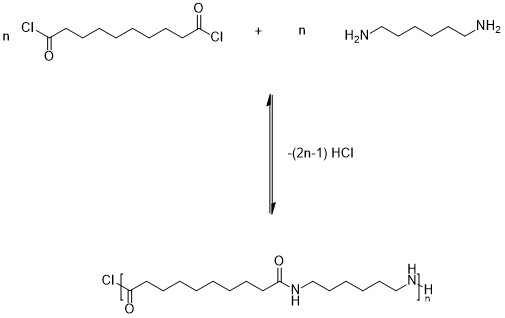
\includegraphics[width=0.8\linewidth]{Abbildungen/Polykondensation.jpg}
    \caption{Reaktionsgleichung der Polykondensation von 1,6-Hexamethylendiamin und Sebacinsäuredichlorid zur Herstellung von Nylon-6,10.}
    \label{fig:Reaktionsgleichung_Granzflächenpolymerisation}
\end{figure}
\subsection{Zusatzfragen}
Zum weiteren Verständnis wurden vier Fragen gestellt, welche beantwortet werden sollen.\par
Die erste Frage ist, wie der Umsatz $p$ und die Reaktionszeit $t$ bei einer autokatalysierten Polykondensation eines Diols und einer Dicarbonsäure in Zusammenhang stehen, und wie sich das experimentell beweisen lässt. Dies lässt sich mit einigen Annahmen herleiten. Erstens wird bei dieser Reaktion angenommen, dass Diol und Dicarbonsäure in äquimolaren Mengen vorliegen, und aufgrund der Stöchiometrie der Reaktion diese auch in äquimolaren Mengen umgesetzt werden. Daher gelten folgende Annahmen.
\begin{equation}
[\mathrm{COOH}]=[\mathrm{OH}]=c    
\nonumber
\end{equation}
\begin{equation}
   -\frac{\mathrm{d}[\mathrm{COOH}]}{\mathrm{d}}= 
   -\frac{\mathrm{d}[\mathrm{OH}]}{\mathrm{d}} 
   \nonumber
\end{equation}
Hierbei gilt auch wieder Gleichung 1.2.
\begin{equation}
-\frac{\mathrm{d}c}{\mathrm{d}t}=k\cdot\mathrm{[K]}\cdot c^2  
\nonumber
\end{equation}
Nun wird diese Differentialgleichung bei Berücksichtigung der gegebenen Annahmen über eine Integration über den gesamten Reaktionszeitraum gelöst. Anschließend wird noch die Definition des Umsatzes $p=\frac{c_\mathrm{0}-c_\mathrm{t}}{c_\mathrm{0}}$ für die Konzentration eingesetzt, um den folgenden Ausdruck zu erhalten.
\begin{equation}
\frac{1}{1-p}=kt [c]_0^2 +1
\nonumber
\end{equation}
Dabei ist zu erkennen, dass der Umsatz abhängig von der Geschwindigkeitskonstante, vergangener Zeit und der Ausgangskonzentration der Monomere ist. Experimentell kann man das bestimmen, indem man nach bestimmten Zeitintervallen einen Teil des Reaktionsvolumens entnimmt und die Polymerisation in dieser Probe terminiert. Der Umsatz lässt sich beispielsweise über das Molekulargewicht per GPC oder über die Konzentration der Carboxylgruppen per IR-Spektroskopie bestimmen.\\
Die zweite Frage ist, wie sich das Molekulargewicht eines Polykondensats steuern lässt und welche Relevanz die Endgruppen darstellen. Dafür gibt es prinzipiell viele Antworten und Möglichkeiten. Die erste wäre die Entfernung des Kondensationsproduktes, wie zum Beispiel Wasser mittels eines Wasserabscheiders, um die Reaktion auf die Produktseite zu verlegen, was zu hohen Molekulargewichten führt. Um niedrigere Molekulargewichte zu erzielen, könnte die Polymerisation vor 100\% Umsatz terminiert werden oder ein Edukt im Überschuss verwendet werden, um nach der Carothers-Gleichung niedrigere Polymerisationsgrade und damit niedrige Molekulargewichte zu erzielen. Bei Polykondensaten bestimmen die Endgruppen maßgebend die chemischen Eigenschaften. Zum Beispiel beeinflussen die Endgruppen die Reaktivität des Polymers für eine Vernetzung oder Funktionalisierung.\\
Die dritte Frage ist, wenn man ein Polykondensat aus einer Dicarbonsäure und Ethylenglykol herstellt, welche Schwierigkeit zu erwarten ist bei einer azeotropen Veresterung mit Toluol als Schlepper. Das Problem hierbei ist, dass der Siedepunkt des Toluol zu niedrig liegt, welcher durch die Bildung eines Azeotrops mit Wasser sich noch weiter verringert.
\newpage
Somit wird eine zu niedrige Temperatur im Reaktionsgefäß erreicht, was zu schlechten Umsätzen führt. Das Problem lässt sich durch die Verwendung eines höher siedenden Lösemittels wie Xylol oder eines Katalysators lösen.\\
Die vierte Frage ist, welche Methoden es gibt um Polyamide darzustellen. Dafür gibt es mehrere Methoden. Die erste ist wie in diesem Versuch mit der Verwendung eines Diamins und einer Dicarbonsäure also der Kondensation eines AA und eines BB Monomers. Die Zweite Methode ist die Kondensation eines AB Monomers in diesem Fall einer Aminosäure. Die letzte Methode ist die Ringöffnungspolymerisation eines Lactams wie etwa $\mathrm{\epsilon}$-Caprolactam. 



\section{Polyaddtionsreaktionen}
\subsection{Lösungspolymerisation}
\subsubsection{Durchführung}
In einem  $\SI{100}{ml}$ Schlenk-Kolben wurde Poly-THF ($\SI{4}{g},\SI{2}{mmol}$, 1 Äq) vorgelegt und unter Stickstoff ausgeheizt. Anschließend wird Toluol-2,4-diisocyanat ($\SI{0,80}{g},\SI{0,66}{ml},\SI{4,6}{mmol}$, 2,3 Äq), trockenes DMF und Dibutylzinnlaurat in DMF ($\SI{4}{ml},\SI{0,01}{\frac{mol}{l}}$) zugegeben. Das Reaktionsgemisch wurde anschließend bei $\SI{80}{\degree}$C für eine Stunde gerührt. Anschließend wurde 1,4-Butandiol ($\SI{0,23}{g},\SI{0,23}{ml},\SI{2,6}{mmol}$) zugegeben und erneut bei $\SI{80}{\degree}$C für zwei Stunden gerührt. Die Polymerlösung wurde langsam in Methanol ($\SI{250}{ml}$) gefällt und anschließend verworfen.
\newpage
\subsubsection{Auswertung}
In Abbildung \ref{fig:Reaktionsgleichung_Lösungspolymerisation} ist die Reaktionsgleichung der Polyaddition von Touluoldiisocyanat, Polytetrahydrofuran und 1,4-Butandiol dargestellt. Zur Erhöhung des Polymerisationsgrades wurde ein Makrodiol (Polytetrahydrofuran) als Edukt gewählt.
\begin{figure}[H]
    \centering
    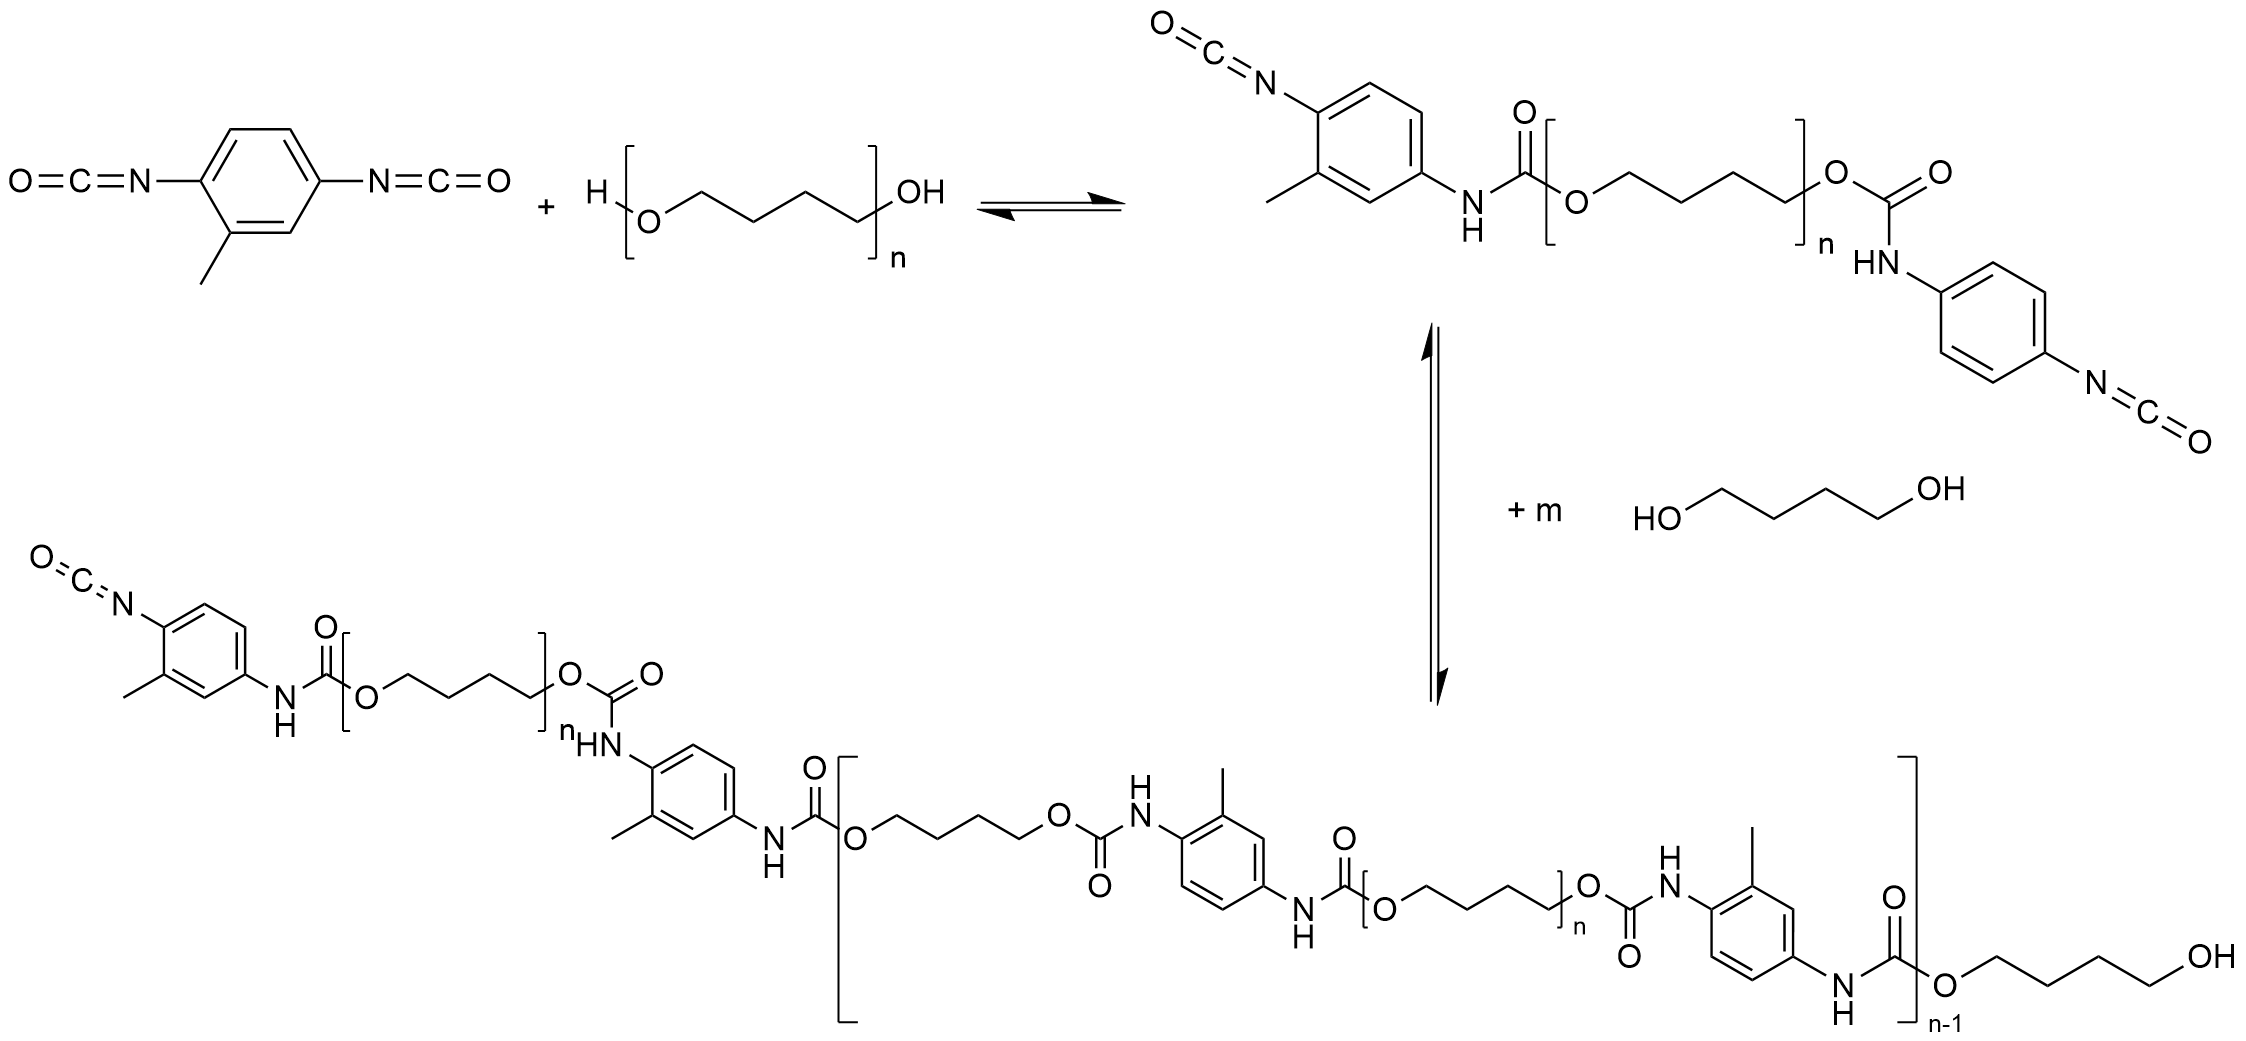
\includegraphics[width=1\linewidth]{Abbildungen/Reaktionsgleichung_Lösungspolymerisation.png}
    \caption{Reaktionsgleichung der Polyadditionsreaktion von TDI, Polytetrahydrofuran und 1,4-Butandiol.}
    \label{fig:Reaktionsgleichung_Lösungspolymerisation}
\end{figure}
Der Reaktionsfortschritt wurde mittels NMR-Spektroskopie untersucht. Dabei wurden im Abstand von jeweils \SI{15}{min} Proben aus dem Reaktionsansatz entnommen. Als Standard wurde Octan zugesetzt. In Tabelle \ref{tab:NMR_Daten} sind die Integralwerte des Standards und der OH-Gruppen im Ansatz dargestellt. Die Werte der Hydroxygruppen müssen hierbei auf den Standard normiert werden. Dies geschieht, wie im folgenden Beispiel für $t=0$ gezeigt. 
\begin{align*}
    I_\text{OH, norm.} = \frac{I_\text{OH}}{I_\text{Octan}} = \frac{\num{16741}}{\num{2305}} = \num{7.2629}
\end{align*}
\newpage

Die übrigen Normierungen berechnen sich analog und sind ebenfalls in Tabelle \ref{tab:NMR_Daten} zusammengefasst.
\begin{table}[H]
    \centering
    \caption{Integralwerte des Octan-Standards, der OH-Gruppen und OH-Gruppen normiert auf den Standard.}
    \begin{tabular}{lccc}
        \hline
        Zeit $t$ [min] & $I_\text{Octan}$ & $I_\text{OH}$ & $I_\text{OH, norm.}$ \\
        \hline\hline
        \num{0}   & \num{2305}  & \num{16741} & \num{7.2629} \\
        \num{15}  & \num{1991}  & \num{13018} & \num{6.5384} \\
        \num{30}  & \num{1770}  & \num{10157} & \num{5.7384} \\
        \num{45}  & \num{2877}  & \num{14625} & \num{5.0834} \\
        \num{60}  & \num{5532}  & \num{24509} & \num{4.4304} \\
        \num{75}  & \num{1106}  & \num{4018}  & \num{3.6329} \\
        \num{90}  & \num{7302}  & \num{20154} & \num{2.7601} \\
        \num{105} & \num{3983}  & \num{8968}  & \num{2.2516} \\
        \num{120} & \num{16374} & \num{23786} & \num{1.4527} \\
        \num{135} & \num{3319}  & \num{2170}  & \num{0.6538} \\
        \hline 
    \end{tabular}
    \label{tab:NMR_Daten}
\end{table}
Aus den normierten Werten für die Hydroxylgruppen lässt sich der Umsatz berechnen. Dies geschieht, wie in Gleichung \ref{eq:Umsatz} gezeigt wird.
\begin{align}
    p(t) = \frac{I_\text{OH, norm.}(0)-I_\text{OH, norm.}(t)}{I_\text{OH, norm.}(0)}
    \label{eq:Umsatz}
\end{align}
Für $t = \SI{15}{min}$ ergibt sich der Umsatz dann wie folgt.
\begin{align}
    p(15) = \frac{\num{7.2629}-\num{6.5384}}{\num{7.2629}} = \num{0.09975}
\end{align}
Basierend auf dem Umsatz kann über die \textit{Carothers}-Gleichung der Polymerisationsgrad bestimmt werden. Dafür wird der Umsatz in Gleichung \ref{eq:Carothers} eingesetzt. Für $t=\SI{15}{min}$ ergibt sich dieser wie folgt. 
\begin{align*}
    P_\text{n}(15)= \frac{1}{1-p(15)} = \frac{1}{1-\num{0.09975}} = \num{1.111}
\end{align*}
Die Umsätze und Polymerisationsgrade der übrigen Zeitpunkte sind in Tabelle \ref{tab:Umsätze,Polymerisationsgrade} zusammengefasst.
\begin{table}[H]
    \centering
     \caption{Zusammenfassung der berechneten Umsätze und Polymerisationsgrade.}
    \begin{tabular}{cccc}
    \hline
    $t$ [min] & $I_\text{OH, norm.}$ & $p(t)$ & $P_\text{n}(t)$ \\
    \hline \hline
    \num{0}   & \num{7.2629} & \num{0}       & \num{1} \\
        \num{15}  & \num{6.5384} & \num{0.0998}  & \num{1.1108} \\
        \num{30}  & \num{5.7384} & \num{0.2099}  & \num{1.2657} \\
        \num{45}  & \num{5.0834} & \num{0.3001}  & \num{1.4287} \\
        \num{60}  & \num{4.4304} & \num{0.3900}  & \num{1.6393} \\
        \num{75}  & \num{3.6329} & \num{0.4998}  & \num{1.9992} \\
        \num{90}  & \num{2.7601} & \num{0.6200}  & \num{2.6314} \\
        \num{105} & \num{2.2516} & \num{0.6900}  & \num{3.2257} \\
        \num{120} & \num{1.4527} & \num{0.8000}  & \num{4.9997} \\
        \num{135} & \num{0.6538} & \num{0.9100}  & \num{11.1086} \\
        \hline
    \end{tabular}
    \label{tab:Umsätze,Polymerisationsgrade}
\end{table}
Wird der Polymerisationsgrad gegen den Umsatz aufgetragen, so ergibt sich der in Abbildung \ref{fig:Auftragung} gezeigte Verlauf.
\begin{figure}[H]
    \centering
    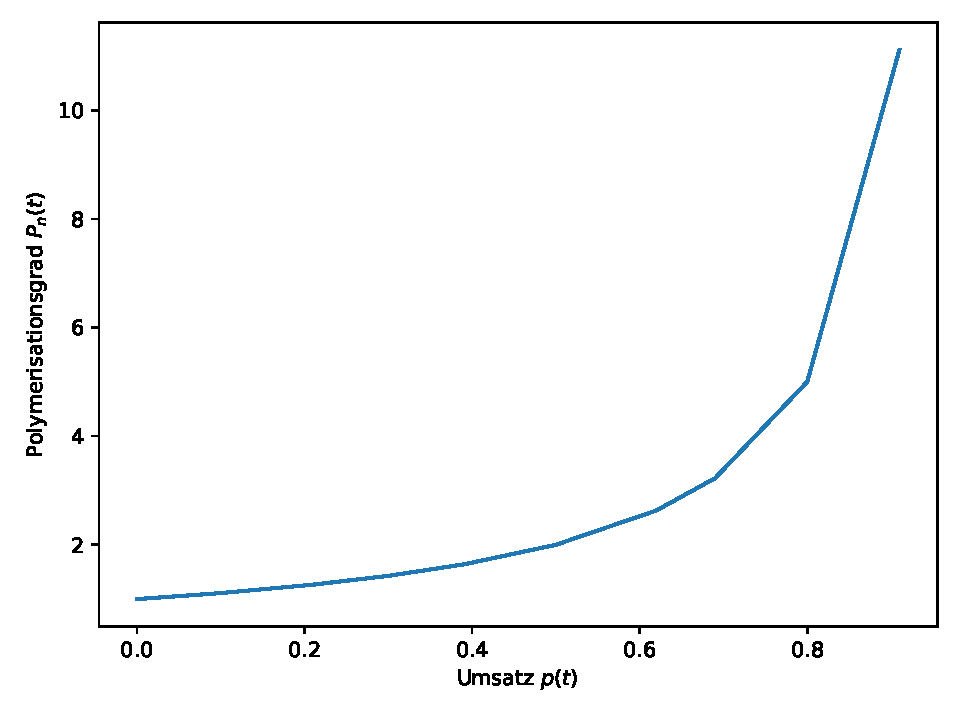
\includegraphics[width=0.9\linewidth]{Abbildungen/Plot.pdf}
    \caption{Auftragung des Polymerisationsgrades gegen den Umsatz.}
    \label{fig:Auftragung}
\end{figure}

\newpage

\subsubsection{Diskussion}
Bei der Synthese des Polyurethans wurde bei der Fällung eine nicht wiegbare Menge an öligem Polymer erhalten. Die geringe Menge beim Fällen lässt sich erklären, dass sich das Polymer zu gut im verwendeten DMF löst und dementsprechend in sehr geringen Mengen ausfiel. Dieses Problem lässt sich durch die Verwendung kleinerer Mengen DMF oder der Verwendung eines schlechteren Lösemittels beheben. Die ölige Eigenschaft des Polymers lässt sich aufgrund eines niedrigen Polymerisationsgrades und der Präsenz von vielen Oligomeren erklären. Dass der Polymerisationsgrad sehr niedrig ausfällt zeigt sich auch in der Auftragung aus Abbildung \ref{fig:Auftragung}. Stufenwachstumsreaktionen benötigen für annehmbare Polymerisationsgrade einen sehr hohen Umsatz (über \SI{99}{\%}). Da dies hier nicht gegeben ist, konnte auch kein Polymer hergestellt werden. Der Umsatz könnte aufgrund ungenauer Einwagen, bzw. ungleicher Stoffmengenverhältnisse der Edukte so niedrig ausgefallen sein.
\subsection{PU-Schaum}
\subsubsection{Durchführung}
Es wurden zwei Ansätze eingewogen. Für den Hartschaum werden Poly(ethylenglycol) 600 (\SI{5}{g}), Glycerin (\SI{1,8}{g}), Natriumdodecylsulfat (\SI{280}{mg}), teilverseiftes Poly(vinylacetat) (\SI{400}{mg}), DMAP (\SI{1}{Spatelspitze}) und Wasser (\SI{2}{g}) eingewogen.\par
Das Weichschaumpolyol besteht aus Poly(ethylenglycol) 600 (\SI{17}{g}), Glycerin (\SI{580}{g}), Natriumdodecylsulfat (\SI{170}{mg}), teilverseiftes Poly(vinylacetat) (\SI{300}{mg}), DMAP (\SI{1}{Spatelspitze}), Silikonöl (\SI{1}{Tropfen}) und Wasser (\SI{2}{g}). Zur Schäumung wird beiden Ansätzen Diisocynat (\SI{10}{mL}) zugesetzt und gerührt.
\subsubsection{Auswertung}
Beide Ansätze schäumten unter Temperaturentwicklung. Der Ansatz des Weichchauemes zeigte hierbei eine stärker exotherme Reaktion. Die unterschiedlichen Eigenschaften der Schäume sind auf die Merkmale der eingesetzten Monomere zurückzuführen. Im Hartschaum sorgt der erhöhte Anteil des Trialkohols Glycerin für eine stärkere Vernetzung der Polymerketten, was dann zu den bekannten mechanischen Eigenschaften führt.
\newpage

\subsection{Zusatzfragen}
In diesem Versuchsteil sollten ebenfalls Fragen beantwortet werden.
Die erste Frage/Aufgabe besteht darin, die Mechanismen der basenkatalysierten oder unkatalysierten Reaktion der folgenden Reaktanden zu formulieren: Isocyanat und Wasser, Isocyanat und Alkohol, Isocyanat und Amin, Isocyanat und Carbonsäure. Diese werden in Abbildung \ref{Wasser Mechanismus}, \ref{Alkohol Mechanismus}, \ref{Amin Mechanismus} und \ref{Carbonsäure Mechanismus} aufgeführt.
\begin{figure}[h!]
\centering
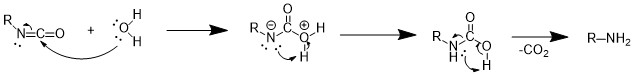
\includegraphics[scale=0.8]{Abbildungen/Wasser Mechanismus.jpg} 
\caption{Reaktionsmechanismus der Reaktion von Isocyanat und Wasser.}  
\label{Wasser Mechanismus}
\end{figure}
\begin{figure}[h!]
\centering
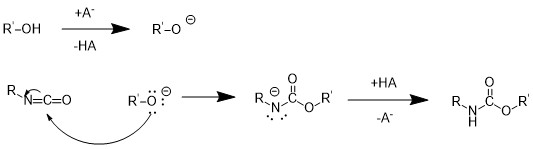
\includegraphics[scale=0.8]{Abbildungen/Alkohol Mechanismus.jpg} 
\caption{Reaktionsmechanismus der basenkatalysierten Reaktion von Isocyanat und Alkohol.}  
\label{Alkohol Mechanismus}
\end{figure}
\begin{figure}[h!]
\centering
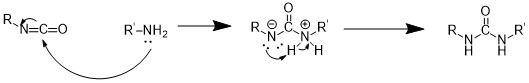
\includegraphics[scale=0.8]{Abbildungen/Amin Mechanismus.jpg } 
\caption{Reaktionsmechanismus der Reaktion von Isocyanat und Amin.}  
\label{Amin Mechanismus}
\end{figure}
\begin{figure}[h!]
\centering
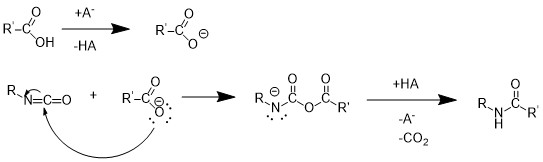
\includegraphics[scale=0.8]{Abbildungen/Carbonsäure Mechanismus.jpg } 
\caption{Reaktionsmechanismus der basenkatalysierten Reaktion von Isocyanat und Carbonsäure.}  
\label{Carbonsäure Mechanismus}
\end{figure}\\

Die zweite Frage ist, warum nicht primäre oder sekundäre Amine für die Katalyse verwendet werden und warum die verwendeten tertiären Amine nicht niedrig sieden dürfen. Weiterhin soll anhand davon erklärt werden, warum die Verwendung von Diethylaminoethanol vorteilhaft ist. 

\newpage
Primäre und sekundäre Amine werden nicht verwendet, weil diese mit den Isocyanat-Gruppen reagieren können, was dazu führt, dass die katalytische Aktivität verloren geht und ungewollte Nebenreaktionen stattfinden. Niedrig siedende tertiäre Amine würden anhand der Reaktionswärme verdampfen und aus dem Schaum entweichen, dadurch sinkt erneut die katalytische Aktivität und die potentiell umweltschädlichen Amine gelangen in die Umwelt. Die Verwendung von Diethylaminoethanol ist vorteilhaft, da die Hydroxylgruppe dazu führt, dass sich dieses in dem Alkohol löst und durch Ausbildung von Wasserstoffbrücken die Siedetemperatur des Diethylaminoethanols relativ hoch ist.\\
Die dritte Aufgabe ist die Reaktionsgleichung eines Isocyanats mit Wasser zu einem Harnstoff aufzuführen. Diese ist in Abbildung \ref{Harnstoff Gleichung} aufgelistet.
\begin{figure}[h!]
\centering
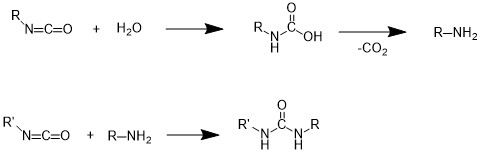
\includegraphics[scale=0.8]{Abbildungen/Harnstoff Gleichung.jpg}  
\caption{Reaktionsgleichung der Reaktion eines Isocyanats und Wasser zu einem Harnstoff.}  
\label{Harnstoff Gleichung}
\end{figure}\\
Die vierte Aufgabe ist die Reaktionsgleichung der Bildung eines Biurets ausgehend von Isocyanaten und Wasser zur Vernetzung aufzuführen. Dies ist in Abbildung \ref{Biuret Gleichung} dargestellt.
\begin{figure}[h!]
\centering
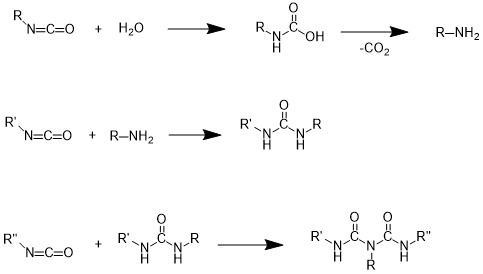
\includegraphics[scale=0.8]{Abbildungen/Biuret Gleichung.jpg} 
\caption{Reaktionsgleichung der Reaktion eines Isocyanats und Wasser zu einem Harnstoff.}  
\label{Biuret Gleichung}
\end{figure}\\
Die fünfte Frage ist, was passiert, wenn die Schäumgeschwindigkeit deutlich größer ist als Polyadditionsgeschwindigkeit bei der Bildung eines PU-Schaums. Bei einer deutlich höheren Schäumingsgeschwindigkeit dehnt sich der Schaum deutlich schneller aus, als sich das Polymer bildet und vernetzt. Das resultiert in in einer geringen mechanischen Stabilität, Festigkeit und Dichte. Wenn die Polyadditionsgeschwindigkeit deutlich höher ist, resultiert das in einem zu festen, kompakten und dichtem Schaum, welcher unter mechanischer Belastung reißen oder brechen könnte.\\
\newpage

Die letzte Frage ist, wie sich Weichschäume und Hartschäume strukturell unterscheiden. Die Antwort darauf ist, dass Weichschäume aus bifunktionellen Monomeren synthetisiert werden. Diese Schäume sind leicht vernetzt und weisen eine geringe Dichte auf. Diese sind auch stark porös, was es ermöglicht, dass Luft durch den Schaum passieren kann. Hartschäume werden aus Monomeren höherer Funktionalität hergestellt. Diese sind stark vernetzt, dicht und nicht Luftdurchlässig.

\printbibliography
\newpage
\end{document}
